\documentclass[tikz]{standalone}
\usepackage{tikz}
\usepackage{circuitikz}

\begin{document}
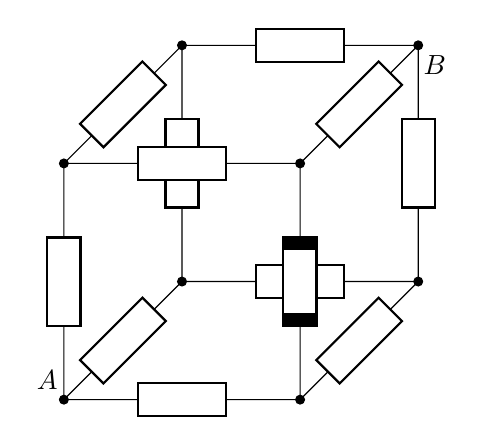
\begin{tikzpicture}[european]
	\draw (0,0) node [left=6pt,above] {$A$} to [R, *-*] (3,0) to [R, -*] (4.5,1.5) to [R, -*] (1.5,1.5) to [R] (0,0)
	(0,3) to [R, *-*] (3,3) to [R, -*] (4.5,4.5) node [right=6pt, below] {$B$} to [R, -*] (1.5,4.5) to [R] (0,3)
	(0,0) to [R] (0,3)
	(3,0) to [R,fill=black] (3,3)
	(4.5,1.5) to [R] (4.5,4.5)
	(1.5,1.5) to [R] (1.5,4.5);
	\draw (2.80,1.1) [draw=none, fill = white] rectangle (3.195,1.9); 
	\draw (1.1,2.805) [draw=none, fill = white] rectangle (1.9,3.195); 
\end{tikzpicture}
\end{document}